\documentclass[]{article}
\usepackage{lmodern}
\usepackage{amssymb,amsmath}
\usepackage{ifxetex,ifluatex}
\usepackage{fixltx2e} \% provides \textsubscript
\ifnum 0\ifxetex 1\fi\ifluatex 1\fi=0 \% if pdftex
  \usepackage[T1]{fontenc}
  \usepackage[utf8]{inputenc}
\else \% if luatex or xelatex
  \ifxetex
    \usepackage{mathspec}
  \else
    \usepackage{fontspec}
  \fi
  \defaultfontfeatures{Ligatures=TeX,Scale=MatchLowercase}
\fi
\% use upquote if available, for straight quotes in verbatim environments
\IfFileExists{upquote.sty}{\usepackage{upquote}}{}
\% use microtype if available
\IfFileExists{microtype.sty}{\%
\usepackage{microtype}
\UseMicrotypeSet[protrusion]{basicmath} \% disable protrusion for tt fonts
}{}
\usepackage[margin=1in]{geometry}
\usepackage{hyperref}
\hypersetup{unicode=true,
            pdftitle={Assignment 6},
            pdfauthor={Kaicheng Luo},
            pdfborder={0 0 0},
            breaklinks=true}
\urlstyle{same}  \% don't use monospace font for urls
\usepackage{color}
\usepackage{fancyvrb}
\newcommand{\VerbBar}{|}
\newcommand{\VERB}{\Verb[commandchars=\\\{\}]}
\DefineVerbatimEnvironment{Highlighting}{Verbatim}{commandchars=\\\{\}}
\% Add ',fontsize=\small' for more characters per line
\usepackage{framed}
\definecolor{shadecolor}{RGB}{248,248,248}
\newenvironment{Shaded}{\begin{snugshade}}{\end{snugshade}}
\newcommand{\KeywordTok}[1]{\textcolor[rgb]{0.13,0.29,0.53}{\textbf{#1}}}
\newcommand{\DataTypeTok}[1]{\textcolor[rgb]{0.13,0.29,0.53}{#1}}
\newcommand{\DecValTok}[1]{\textcolor[rgb]{0.00,0.00,0.81}{#1}}
\newcommand{\BaseNTok}[1]{\textcolor[rgb]{0.00,0.00,0.81}{#1}}
\newcommand{\FloatTok}[1]{\textcolor[rgb]{0.00,0.00,0.81}{#1}}
\newcommand{\ConstantTok}[1]{\textcolor[rgb]{0.00,0.00,0.00}{#1}}
\newcommand{\CharTok}[1]{\textcolor[rgb]{0.31,0.60,0.02}{#1}}
\newcommand{\SpecialCharTok}[1]{\textcolor[rgb]{0.00,0.00,0.00}{#1}}
\newcommand{\StringTok}[1]{\textcolor[rgb]{0.31,0.60,0.02}{#1}}
\newcommand{\VerbatimStringTok}[1]{\textcolor[rgb]{0.31,0.60,0.02}{#1}}
\newcommand{\SpecialStringTok}[1]{\textcolor[rgb]{0.31,0.60,0.02}{#1}}
\newcommand{\ImportTok}[1]{#1}
\newcommand{\CommentTok}[1]{\textcolor[rgb]{0.56,0.35,0.01}{\textit{#1}}}
\newcommand{\DocumentationTok}[1]{\textcolor[rgb]{0.56,0.35,0.01}{\textbf{\textit{#1}}}}
\newcommand{\AnnotationTok}[1]{\textcolor[rgb]{0.56,0.35,0.01}{\textbf{\textit{#1}}}}
\newcommand{\CommentVarTok}[1]{\textcolor[rgb]{0.56,0.35,0.01}{\textbf{\textit{#1}}}}
\newcommand{\OtherTok}[1]{\textcolor[rgb]{0.56,0.35,0.01}{#1}}
\newcommand{\FunctionTok}[1]{\textcolor[rgb]{0.00,0.00,0.00}{#1}}
\newcommand{\VariableTok}[1]{\textcolor[rgb]{0.00,0.00,0.00}{#1}}
\newcommand{\ControlFlowTok}[1]{\textcolor[rgb]{0.13,0.29,0.53}{\textbf{#1}}}
\newcommand{\OperatorTok}[1]{\textcolor[rgb]{0.81,0.36,0.00}{\textbf{#1}}}
\newcommand{\BuiltInTok}[1]{#1}
\newcommand{\ExtensionTok}[1]{#1}
\newcommand{\PreprocessorTok}[1]{\textcolor[rgb]{0.56,0.35,0.01}{\textit{#1}}}
\newcommand{\AttributeTok}[1]{\textcolor[rgb]{0.77,0.63,0.00}{#1}}
\newcommand{\RegionMarkerTok}[1]{#1}
\newcommand{\InformationTok}[1]{\textcolor[rgb]{0.56,0.35,0.01}{\textbf{\textit{#1}}}}
\newcommand{\WarningTok}[1]{\textcolor[rgb]{0.56,0.35,0.01}{\textbf{\textit{#1}}}}
\newcommand{\AlertTok}[1]{\textcolor[rgb]{0.94,0.16,0.16}{#1}}
\newcommand{\ErrorTok}[1]{\textcolor[rgb]{0.64,0.00,0.00}{\textbf{#1}}}
\newcommand{\NormalTok}[1]{#1}
\usepackage{graphicx}
\% grffile has become a legacy package: https://ctan.org/pkg/grffile
\IfFileExists{grffile.sty}{\%
\usepackage{grffile}
}{}
\makeatletter
\def\maxwidth{\ifdim\Gin@nat@width>\linewidth\linewidth\else\Gin@nat@width\fi}
\def\maxheight{\ifdim\Gin@nat@height>\textheight\textheight\else\Gin@nat@height\fi}
\makeatother
\% Scale images if necessary, so that they will not overflow the page
\% margins by default, and it is still possible to overwrite the defaults
\% using explicit options in \includegraphics[width, height, ...]{}
\setkeys{Gin}{width=\maxwidth,height=\maxheight,keepaspectratio}
\IfFileExists{parskip.sty}{\%
\usepackage{parskip}
}{\% else
\setlength{\parindent}{0pt}
\setlength{\parskip}{6pt plus 2pt minus 1pt}
}
\setlength{\emergencystretch}{3em}  \% prevent overfull lines
\providecommand{\tightlist}{\%
  \setlength{\itemsep}{0pt}\setlength{\parskip}{0pt}}
\setcounter{secnumdepth}{0}
\% Redefines (sub)paragraphs to behave more like sections
\ifx\paragraph\undefined\else
\let\oldparagraph\paragraph
\renewcommand{\paragraph}[1]{\oldparagraph{#1}\mbox{}}
\fi
\ifx\subparagraph\undefined\else
\let\oldsubparagraph\subparagraph
\renewcommand{\subparagraph}[1]{\oldsubparagraph{#1}\mbox{}}
\fi

\%\%\% Use protect on footnotes to avoid problems with footnotes in titles
\let\rmarkdownfootnote\footnote\%
\def\footnote{\protect\rmarkdownfootnote}

\%\%\% Change title format to be more compact
\usepackage{titling}

\% Create subtitle command for use in maketitle
\providecommand{\subtitle}[1]{
  \posttitle{
    \begin{center}\large#1\end{center}
    }
}

\setlength{\droptitle}{-2em}

  \title{Assignment 6}
    \pretitle{\vspace{\droptitle}\centering\huge}
  \posttitle{\par}
    \author{Kaicheng Luo}
    \preauthor{\centering\large\emph}
  \postauthor{\par}
      \predate{\centering\large\emph}
  \postdate{\par}
    \date{2019/11/28}


\begin{document}
\maketitle

\section*{Problem 1}

An example of proper IV data is

\begin{Shaded}
\begin{Highlighting}[]
\NormalTok{data <-}\StringTok{ }\KeywordTok{data.frame}\NormalTok{(}\StringTok{"Z"}\NormalTok{ =}\StringTok{ }\KeywordTok{c}\NormalTok{(}\DecValTok{1}\NormalTok{,}\DecValTok{1}\NormalTok{,}\DecValTok{0}\NormalTok{,}\DecValTok{0}\NormalTok{), }\StringTok{"D"}\NormalTok{ =}\StringTok{ }\KeywordTok{c}\NormalTok{(}\DecValTok{1}\NormalTok{,}\DecValTok{1}\NormalTok{,}\DecValTok{0}\NormalTok{,}\DecValTok{0}\NormalTok{), }\StringTok{"Y"}\NormalTok{ =}\StringTok{ }\KeywordTok{c}\NormalTok{(}\DecValTok{1}\NormalTok{,}\DecValTok{1}\NormalTok{,}\DecValTok{0}\NormalTok{,}\DecValTok{0}\NormalTok{))}
\NormalTok{data}
\end{Highlighting}
\end{Shaded}

\begin{verbatim}
##   Z D Y
## 1 1 1 1
## 2 1 1 1
## 3 0 0 0
## 4 0 0 0
\end{verbatim}

\begin{Shaded}
\begin{Highlighting}[]
\NormalTok{Q <-}\StringTok{ }\KeywordTok{cbind}\NormalTok{(data}\OperatorTok{\$}\NormalTok{D }\OperatorTok{*}\StringTok{ }\NormalTok{data}\OperatorTok{\$}\NormalTok{Y, data}\OperatorTok{\$}\NormalTok{D}\OperatorTok{*}\NormalTok{(}\DecValTok{1} \OperatorTok{-}\StringTok{ }\NormalTok{data}\OperatorTok{\$}\NormalTok{Y), data}\OperatorTok{\$}\NormalTok{Y}\OperatorTok{*}\NormalTok{(}\DecValTok{1}\OperatorTok{-}\NormalTok{data}\OperatorTok{\$}\NormalTok{D), data}\OperatorTok{\$}\NormalTok{D}\OperatorTok{+}\NormalTok{data}\OperatorTok{\$}\NormalTok{Y }\OperatorTok{-}\StringTok{ }\NormalTok{data}\OperatorTok{\$}\NormalTok{D }\OperatorTok{*}\StringTok{ }\NormalTok{data}\OperatorTok{\$}\NormalTok{Y)}
\KeywordTok{mean}\NormalTok{(Q[}\DecValTok{1}\OperatorTok{:}\DecValTok{2}\NormalTok{,}\DecValTok{1}\NormalTok{]) }\OperatorTok{-}\StringTok{ }\KeywordTok{mean}\NormalTok{(Q[}\DecValTok{3}\OperatorTok{:}\DecValTok{4}\NormalTok{,}\DecValTok{1}\NormalTok{])}
\end{Highlighting}
\end{Shaded}

\begin{verbatim}
## [1] 1
\end{verbatim}

\begin{Shaded}
\begin{Highlighting}[]
\KeywordTok{mean}\NormalTok{(Q[}\DecValTok{1}\OperatorTok{:}\DecValTok{2}\NormalTok{,}\DecValTok{2}\NormalTok{]) }\OperatorTok{-}\StringTok{ }\KeywordTok{mean}\NormalTok{(Q[}\DecValTok{3}\OperatorTok{:}\DecValTok{4}\NormalTok{,}\DecValTok{2}\NormalTok{])}
\end{Highlighting}
\end{Shaded}

\begin{verbatim}
## [1] 0
\end{verbatim}

\begin{Shaded}
\begin{Highlighting}[]
\KeywordTok{mean}\NormalTok{(Q[}\DecValTok{1}\OperatorTok{:}\DecValTok{2}\NormalTok{,}\DecValTok{3}\NormalTok{]) }\OperatorTok{-}\StringTok{ }\KeywordTok{mean}\NormalTok{(Q[}\DecValTok{3}\OperatorTok{:}\DecValTok{4}\NormalTok{,}\DecValTok{3}\NormalTok{])}
\end{Highlighting}
\end{Shaded}

\begin{verbatim}
## [1] 0
\end{verbatim}

\begin{Shaded}
\begin{Highlighting}[]
\KeywordTok{mean}\NormalTok{(Q[}\DecValTok{1}\OperatorTok{:}\DecValTok{2}\NormalTok{,}\DecValTok{4}\NormalTok{]) }\OperatorTok{-}\StringTok{ }\KeywordTok{mean}\NormalTok{(Q[}\DecValTok{3}\OperatorTok{:}\DecValTok{4}\NormalTok{,}\DecValTok{4}\NormalTok{])}
\end{Highlighting}
\end{Shaded}

\begin{verbatim}
## [1] 1
\end{verbatim}

An example of improper IV data is

\begin{Shaded}
\begin{Highlighting}[]
\NormalTok{data <-}\StringTok{ }\KeywordTok{data.frame}\NormalTok{(}\StringTok{"Z"}\NormalTok{ =}\StringTok{ }\KeywordTok{c}\NormalTok{(}\DecValTok{1}\NormalTok{,}\DecValTok{1}\NormalTok{,}\DecValTok{0}\NormalTok{,}\DecValTok{0}\NormalTok{), }\StringTok{"D"}\NormalTok{ =}\StringTok{ }\KeywordTok{c}\NormalTok{(}\DecValTok{1}\NormalTok{,}\DecValTok{1}\NormalTok{,}\DecValTok{1}\NormalTok{,}\DecValTok{0}\NormalTok{), }\StringTok{"Y"}\NormalTok{ =}\StringTok{ }\KeywordTok{c}\NormalTok{(}\DecValTok{1}\NormalTok{,}\DecValTok{1}\NormalTok{,}\DecValTok{0}\NormalTok{,}\DecValTok{0}\NormalTok{))}
\NormalTok{data}
\end{Highlighting}
\end{Shaded}

\begin{verbatim}
##   Z D Y
## 1 1 1 1
## 2 1 1 1
## 3 0 1 0
## 4 0 0 0
\end{verbatim}

\begin{Shaded}
\begin{Highlighting}[]
\NormalTok{Q <-}\StringTok{ }\KeywordTok{cbind}\NormalTok{(data}\OperatorTok{\$}\NormalTok{D }\OperatorTok{*}\StringTok{ }\NormalTok{data}\OperatorTok{\$}\NormalTok{Y, data}\OperatorTok{\$}\NormalTok{D}\OperatorTok{*}\NormalTok{(}\DecValTok{1} \OperatorTok{-}\StringTok{ }\NormalTok{data}\OperatorTok{\$}\NormalTok{Y), data}\OperatorTok{\$}\NormalTok{Y}\OperatorTok{*}\NormalTok{(}\DecValTok{1}\OperatorTok{-}\NormalTok{data}\OperatorTok{\$}\NormalTok{D), data}\OperatorTok{\$}\NormalTok{D}\OperatorTok{+}\NormalTok{data}\OperatorTok{\$}\NormalTok{Y }\OperatorTok{-}\StringTok{ }\NormalTok{data}\OperatorTok{\$}\NormalTok{D }\OperatorTok{*}\StringTok{ }\NormalTok{data}\OperatorTok{\$}\NormalTok{Y)}
\KeywordTok{mean}\NormalTok{(Q[}\DecValTok{1}\OperatorTok{:}\DecValTok{2}\NormalTok{,}\DecValTok{1}\NormalTok{]) }\OperatorTok{-}\StringTok{ }\KeywordTok{mean}\NormalTok{(Q[}\DecValTok{3}\OperatorTok{:}\DecValTok{4}\NormalTok{,}\DecValTok{1}\NormalTok{])}
\end{Highlighting}
\end{Shaded}

\begin{verbatim}
## [1] 1
\end{verbatim}

\begin{Shaded}
\begin{Highlighting}[]
\KeywordTok{mean}\NormalTok{(Q[}\DecValTok{1}\OperatorTok{:}\DecValTok{2}\NormalTok{,}\DecValTok{2}\NormalTok{]) }\OperatorTok{-}\StringTok{ }\KeywordTok{mean}\NormalTok{(Q[}\DecValTok{3}\OperatorTok{:}\DecValTok{4}\NormalTok{,}\DecValTok{2}\NormalTok{])}
\end{Highlighting}
\end{Shaded}

\begin{verbatim}
## [1] -0.5
\end{verbatim}

\begin{Shaded}
\begin{Highlighting}[]
\KeywordTok{mean}\NormalTok{(Q[}\DecValTok{1}\OperatorTok{:}\DecValTok{2}\NormalTok{,}\DecValTok{3}\NormalTok{]) }\OperatorTok{-}\StringTok{ }\KeywordTok{mean}\NormalTok{(Q[}\DecValTok{3}\OperatorTok{:}\DecValTok{4}\NormalTok{,}\DecValTok{3}\NormalTok{])}
\end{Highlighting}
\end{Shaded}

\begin{verbatim}
## [1] 0
\end{verbatim}

\begin{Shaded}
\begin{Highlighting}[]
\KeywordTok{mean}\NormalTok{(Q[}\DecValTok{1}\OperatorTok{:}\DecValTok{2}\NormalTok{,}\DecValTok{4}\NormalTok{]) }\OperatorTok{-}\StringTok{ }\KeywordTok{mean}\NormalTok{(Q[}\DecValTok{3}\OperatorTok{:}\DecValTok{4}\NormalTok{,}\DecValTok{4}\NormalTok{])}
\end{Highlighting}
\end{Shaded}

\begin{verbatim}
## [1] 0.5
\end{verbatim}

\section*{Problem 3}

Some sketch about our data: there are many tricky properties in our
data. For missing values, we interpolate the income and work length data
as zero for those unemployed. This helps us avoid dropping so many NA
values in our observations. The total observations dropped is 354 out of
10454 (already dropping those with no response).

\begin{Shaded}
\begin{Highlighting}[]
\NormalTok{xdat <-}\StringTok{ }\KeywordTok{read.csv}\NormalTok{(}\StringTok{"X.csv"}\NormalTok{, }\DataTypeTok{header =}\NormalTok{ T, }\DataTypeTok{sep =} \StringTok{","}\NormalTok{)}
\NormalTok{ydat <-}\StringTok{ }\KeywordTok{read.csv}\NormalTok{(}\DataTypeTok{file=}\StringTok{"Y.csv"}\NormalTok{, }\DataTypeTok{header =} \OtherTok{TRUE}\NormalTok{, }\DataTypeTok{sep =} \StringTok{","}\NormalTok{)}
\NormalTok{dat <-}\StringTok{ }\KeywordTok{bind_cols}\NormalTok{(xdat, ydat)}
\KeywordTok{names}\NormalTok{(dat)}
\end{Highlighting}
\end{Shaded}

\begin{verbatim}
##  [1] "const"     "wgt"       "female"    "age"       "haschld"   "educ"     
##  [7] "educ.m"    "educ.f"    "currjob"   "mosinjob"  "yr_work1"  "earn_yr"  
## [13] "white"     "partnered" "evarrst"   "p_inc"     "hh_inc"    "R.educ.m" 
## [19] "R.educ.f"  "R.hh_inc"  "I.educ.m"  "I.educ.f"  "I.hh_inc"  "ID"       
## [25] "wgt1"      "assign"    "treat"     "r52"       "work52"    "y52"      
## [31] "h52"       "w52"       "r130"      "work130"   "y130"      "h130"     
## [37] "w130"      "r208"      "work208"   "y208"      "h208"      "w208"     
## [43] "TOTHRSW"   "EARNY4"
\end{verbatim}

\begin{Shaded}
\begin{Highlighting}[]
\NormalTok{dat <-}\StringTok{ }\NormalTok{dat }\OperatorTok{\%>\%}
\StringTok{  }\KeywordTok{filter}\NormalTok{(r52 }\OperatorTok{==}\StringTok{ }\DecValTok{1} \OperatorTok{&}\StringTok{ }\NormalTok{r130 }\OperatorTok{==}\StringTok{ }\DecValTok{1} \OperatorTok{&}\StringTok{ }\NormalTok{r208 }\OperatorTok{==}\StringTok{ }\DecValTok{1}\NormalTok{) }\OperatorTok{\%>\%}
\StringTok{  }\KeywordTok{mutate}\NormalTok{(}\DataTypeTok{w52 =} \KeywordTok{ifelse}\NormalTok{(}\KeywordTok{is.na}\NormalTok{(w52), }\DecValTok{0}\NormalTok{, w52)) }\OperatorTok{\%>\%}
\StringTok{  }\KeywordTok{mutate}\NormalTok{(}\DataTypeTok{w130 =} \KeywordTok{ifelse}\NormalTok{(}\KeywordTok{is.na}\NormalTok{(w130), }\DecValTok{0}\NormalTok{, w130)) }\OperatorTok{\%>\%}
\StringTok{  }\KeywordTok{mutate}\NormalTok{(}\DataTypeTok{w208 =} \KeywordTok{ifelse}\NormalTok{(}\KeywordTok{is.na}\NormalTok{(w208), }\DecValTok{0}\NormalTok{, w208))}
\KeywordTok{sum}\NormalTok{(}\KeywordTok{is.na}\NormalTok{(dat))}
\end{Highlighting}
\end{Shaded}

\begin{verbatim}
## [1] 354
\end{verbatim}

\begin{Shaded}
\begin{Highlighting}[]
\NormalTok{dat <-}\StringTok{ }\KeywordTok{na.omit}\NormalTok{(dat)}
\CommentTok{# 1. Without Covariates}
\NormalTok{Z <-}\StringTok{ }\NormalTok{dat }\OperatorTok{\%>\%}
\StringTok{  }\KeywordTok{select}\NormalTok{(assign)}
\NormalTok{D <-}\StringTok{ }\NormalTok{dat }\OperatorTok{\%>\%}
\StringTok{  }\KeywordTok{select}\NormalTok{(treat)}
\NormalTok{Y <-}\StringTok{ }\NormalTok{dat[,}\DecValTok{39}\OperatorTok{:}\DecValTok{44}\NormalTok{]}
\NormalTok{X <-}\StringTok{ }\NormalTok{dat[,}\DecValTok{2}\OperatorTok{:}\DecValTok{23}\NormalTok{]}
\end{Highlighting}
\end{Shaded}

\begin{Shaded}
\begin{Highlighting}[]
\NormalTok{IV_Wald =}\StringTok{ }\ControlFlowTok{function}\NormalTok{(Z, D, Y)}
\NormalTok{\{}
\NormalTok{       tau_D =}\StringTok{ }\KeywordTok{mean}\NormalTok{(D[Z}\OperatorTok{==}\DecValTok{1}\NormalTok{]) }\OperatorTok{-}\StringTok{ }\KeywordTok{mean}\NormalTok{(D[Z}\OperatorTok{==}\DecValTok{0}\NormalTok{])}
\NormalTok{       tau_Y =}\StringTok{ }\KeywordTok{mean}\NormalTok{(Y[Z}\OperatorTok{==}\DecValTok{1}\NormalTok{]) }\OperatorTok{-}\StringTok{ }\KeywordTok{mean}\NormalTok{(Y[Z}\OperatorTok{==}\DecValTok{0}\NormalTok{])}
\NormalTok{       CACE  =}\StringTok{ }\NormalTok{tau_Y}\OperatorTok{/}\NormalTok{tau_D}
       
       \KeywordTok{return}\NormalTok{(}\KeywordTok{list}\NormalTok{(}\DataTypeTok{tau_D =}\NormalTok{ tau_D, }\DataTypeTok{tau_Y =}\NormalTok{ tau_Y,}
                   \DataTypeTok{CACE  =}\NormalTok{ CACE))}
\NormalTok{\}}

\NormalTok{## IV se via the delta method}
\NormalTok{IV_Wald_delta =}\StringTok{ }\ControlFlowTok{function}\NormalTok{(Z, D, Y)}
\NormalTok{\{}
\NormalTok{       est         =}\StringTok{ }\KeywordTok{IV_Wald}\NormalTok{(Z, D, Y)}
\NormalTok{       AdjustedY   =}\StringTok{ }\NormalTok{Y }\OperatorTok{-}\StringTok{ }\NormalTok{D}\OperatorTok{*}\NormalTok{est}\OperatorTok{\$}\NormalTok{CACE}
\NormalTok{       VarAdj      =}\StringTok{ }\KeywordTok{var}\NormalTok{(AdjustedY[Z}\OperatorTok{==}\DecValTok{1}\NormalTok{])}\OperatorTok{/}\KeywordTok{sum}\NormalTok{(Z) }\OperatorTok{+}\StringTok{ }
\StringTok{                          }\KeywordTok{var}\NormalTok{(AdjustedY[Z}\OperatorTok{==}\DecValTok{0}\NormalTok{])}\OperatorTok{/}\KeywordTok{sum}\NormalTok{(}\DecValTok{1} \OperatorTok{-}\StringTok{ }\NormalTok{Z)}
       \KeywordTok{return}\NormalTok{(}\KeywordTok{sqrt}\NormalTok{(VarAdj)}\OperatorTok{/}\KeywordTok{abs}\NormalTok{(est}\OperatorTok{\$}\NormalTok{tau_D))}
\NormalTok{\}}
\end{Highlighting}
\end{Shaded}

\begin{Shaded}
\begin{Highlighting}[]
\CommentTok{# IV wald estimation without covariates}
\ControlFlowTok{for}\NormalTok{ (i }\ControlFlowTok{in} \DecValTok{1}\OperatorTok{:}\DecValTok{6}\NormalTok{)}
\NormalTok{\{}
\NormalTok{  est =}\StringTok{ }\KeywordTok{IV_Wald}\NormalTok{(Z, D, Y[,i])}
\NormalTok{  estVar =}\StringTok{ }\KeywordTok{IV_Wald_delta}\NormalTok{(Z, D, Y[,i])}
  \KeywordTok{print}\NormalTok{(}\KeywordTok{paste}\NormalTok{(}\StringTok{"The (Wald) point estimate of the treatment effect for "}\NormalTok{, }\KeywordTok{colnames}\NormalTok{(Y)[i] ,}\StringTok{" is "}\NormalTok{, est}\OperatorTok{\$}\NormalTok{CACE, }\StringTok{" and the confidence interval is ["}\NormalTok{, est}\OperatorTok{\$}\NormalTok{CACE }\OperatorTok{-}\StringTok{ }\FloatTok{1.96}\OperatorTok{*}\NormalTok{estVar,}\StringTok{","}\NormalTok{,est}\OperatorTok{\$}\NormalTok{CACE }\OperatorTok{+}\StringTok{ }\FloatTok{1.96}\OperatorTok{*}\NormalTok{estVar,}\StringTok{"]"}\NormalTok{, }\DataTypeTok{sep =} \StringTok{""}\NormalTok{))}
\NormalTok{\}}
\end{Highlighting}
\end{Shaded}

\begin{verbatim}
## [1] "The (Wald) point estimate of the treatment effect for work208 is 0.0505451407972023 and the confidence interval is [0.02255830088846,0.0785319807059446]"
## [1] "The (Wald) point estimate of the treatment effect for y208 is 29.3200533263004 and the confidence interval is [15.2890735763043,43.3510330762966]"
## [1] "The (Wald) point estimate of the treatment effect for h208 is 2.25222199510049 and the confidence interval is [0.817894623514175,3.68654936668681]"
## [1] "The (Wald) point estimate of the treatment effect for w208 is 0.580465717577646 and the confidence interval is [0.29297306566072,0.867958369494572]"
## [1] "The (Wald) point estimate of the treatment effect for TOTHRSW is -1.24813761309078 and the confidence interval is [-2.04287051604833,-0.453404710133226]"
## [1] "The (Wald) point estimate of the treatment effect for EARNY4 is 19.0338473074643 and the confidence interval is [7.97433630102675,30.0933583139019]"
\end{verbatim}

\begin{Shaded}
\begin{Highlighting}[]
\NormalTok{IV_Lin =}\StringTok{ }\ControlFlowTok{function}\NormalTok{(Z, D, Y, X)}
\NormalTok{\{}
\NormalTok{  X =}\StringTok{ }\KeywordTok{as.matrix}\NormalTok{(X)}
\NormalTok{  D =}\StringTok{ }\KeywordTok{as.matrix}\NormalTok{(D)}
\NormalTok{  Y =}\StringTok{ }\KeywordTok{as.matrix}\NormalTok{(Y)}
\NormalTok{  Z =}\StringTok{ }\KeywordTok{as.matrix}\NormalTok{(Z)}
\NormalTok{  tau_D =}\StringTok{ }\KeywordTok{lm}\NormalTok{(D }\OperatorTok{~}\StringTok{ }\NormalTok{Z }\OperatorTok{+}\StringTok{ }\NormalTok{X }\OperatorTok{+}\StringTok{ }\NormalTok{Z}\OperatorTok{*}\NormalTok{X)}\OperatorTok{\$}\NormalTok{coef[}\DecValTok{2}\NormalTok{]}
\NormalTok{  tau_Y =}\StringTok{ }\KeywordTok{lm}\NormalTok{(Y }\OperatorTok{~}\StringTok{ }\NormalTok{Z }\OperatorTok{+}\StringTok{ }\NormalTok{X }\OperatorTok{+}\StringTok{ }\NormalTok{Z}\OperatorTok{*}\NormalTok{X)}\OperatorTok{\$}\NormalTok{coef[}\DecValTok{2}\NormalTok{]}
  \KeywordTok{names}\NormalTok{(tau_D) =}\StringTok{ }\OtherTok{NULL}
  \KeywordTok{names}\NormalTok{(tau_Y) =}\StringTok{ }\OtherTok{NULL}
\NormalTok{  CACE  =}\StringTok{ }\NormalTok{tau_Y}\OperatorTok{/}\NormalTok{tau_D}
  
  \KeywordTok{return}\NormalTok{(}\KeywordTok{list}\NormalTok{(}\DataTypeTok{tau_D =}\NormalTok{ tau_D, }\DataTypeTok{tau_Y =}\NormalTok{ tau_Y,}
              \DataTypeTok{CACE  =}\NormalTok{ CACE))}
\NormalTok{\}}

\NormalTok{## IV_adj se via the delta method}
\NormalTok{IV_Lin_delta =}\StringTok{ }\ControlFlowTok{function}\NormalTok{(Z, D, Y, X)}
\NormalTok{\{}
\NormalTok{  X =}\StringTok{ }\KeywordTok{as.matrix}\NormalTok{(X)}
\NormalTok{  D =}\StringTok{ }\KeywordTok{as.matrix}\NormalTok{(D)}
\NormalTok{  Y =}\StringTok{ }\KeywordTok{as.matrix}\NormalTok{(Y)}
\NormalTok{  Z =}\StringTok{ }\KeywordTok{as.matrix}\NormalTok{(Z)}
\NormalTok{  est    =}\StringTok{ }\KeywordTok{IV_Lin}\NormalTok{(Z, D, Y, X)}
  
\NormalTok{  betaY1 =}\StringTok{ }\KeywordTok{lm}\NormalTok{(Y }\OperatorTok{~}\StringTok{ }\NormalTok{X, }\DataTypeTok{subset =}\NormalTok{ (Z }\OperatorTok{==}\StringTok{ }\DecValTok{1}\NormalTok{))}\OperatorTok{\$}\NormalTok{coef[}\OperatorTok{-}\DecValTok{1}\NormalTok{]}
\NormalTok{  betaY0 =}\StringTok{ }\KeywordTok{lm}\NormalTok{(Y }\OperatorTok{~}\StringTok{ }\NormalTok{X, }\DataTypeTok{subset =}\NormalTok{ (Z }\OperatorTok{==}\StringTok{ }\DecValTok{0}\NormalTok{))}\OperatorTok{\$}\NormalTok{coef[}\OperatorTok{-}\DecValTok{1}\NormalTok{]}
\NormalTok{  betaD1 =}\StringTok{ }\KeywordTok{lm}\NormalTok{(D }\OperatorTok{~}\StringTok{ }\NormalTok{X, }\DataTypeTok{subset =}\NormalTok{ (Z }\OperatorTok{==}\StringTok{ }\DecValTok{1}\NormalTok{))}\OperatorTok{\$}\NormalTok{coef[}\OperatorTok{-}\DecValTok{1}\NormalTok{]}
\NormalTok{  betaD0 =}\StringTok{ }\KeywordTok{lm}\NormalTok{(D }\OperatorTok{~}\StringTok{ }\NormalTok{X, }\DataTypeTok{subset =}\NormalTok{ (Z }\OperatorTok{==}\StringTok{ }\DecValTok{0}\NormalTok{))}\OperatorTok{\$}\NormalTok{coef[}\OperatorTok{-}\DecValTok{1}\NormalTok{]}
  
\NormalTok{  AdjustedY1   =}\StringTok{ }\NormalTok{Y }\OperatorTok{-}\StringTok{ }\NormalTok{X}\OperatorTok{\%*\%}\NormalTok{betaY1 }\OperatorTok{-}\StringTok{ }
\StringTok{                     }\NormalTok{(D }\OperatorTok{-}\StringTok{ }\NormalTok{X}\OperatorTok{\%*\%}\NormalTok{betaD1)}\OperatorTok{*}\NormalTok{est}\OperatorTok{\$}\NormalTok{CACE}
\NormalTok{  AdjustedY0   =}\StringTok{ }\NormalTok{Y }\OperatorTok{-}\StringTok{ }\NormalTok{X}\OperatorTok{\%*\%}\NormalTok{betaY0 }\OperatorTok{-}\StringTok{ }
\StringTok{                     }\NormalTok{(D }\OperatorTok{-}\StringTok{ }\NormalTok{X}\OperatorTok{\%*\%}\NormalTok{betaD0)}\OperatorTok{*}\NormalTok{est}\OperatorTok{\$}\NormalTok{CACE}
\NormalTok{  VarAdj       =}\StringTok{ }\KeywordTok{var}\NormalTok{(AdjustedY1[Z}\OperatorTok{==}\DecValTok{1}\NormalTok{])}\OperatorTok{/}\KeywordTok{sum}\NormalTok{(Z) }\OperatorTok{+}\StringTok{ }
\StringTok{                     }\KeywordTok{var}\NormalTok{(AdjustedY0[Z}\OperatorTok{==}\DecValTok{0}\NormalTok{])}\OperatorTok{/}\KeywordTok{sum}\NormalTok{(}\DecValTok{1} \OperatorTok{-}\StringTok{ }\NormalTok{Z)}
  
  \KeywordTok{return}\NormalTok{(}\KeywordTok{sqrt}\NormalTok{(VarAdj)}\OperatorTok{/}\KeywordTok{abs}\NormalTok{(est}\OperatorTok{\$}\NormalTok{tau_D))}
\NormalTok{\}}
\end{Highlighting}
\end{Shaded}

\begin{Shaded}
\begin{Highlighting}[]
\CommentTok{# 2. With Covariates}
\CommentTok{# IV wald estimation without covariates}
\ControlFlowTok{for}\NormalTok{ (i }\ControlFlowTok{in} \DecValTok{1}\OperatorTok{:}\DecValTok{6}\NormalTok{)}
\NormalTok{\{}
\NormalTok{  est =}\StringTok{ }\KeywordTok{IV_Lin}\NormalTok{(Z, D, Y[,i], X)}
\NormalTok{  estVar =}\StringTok{ }\KeywordTok{IV_Lin_delta}\NormalTok{(Z, D, Y[,i], X)}
  \KeywordTok{print}\NormalTok{(}\KeywordTok{paste}\NormalTok{(}\StringTok{"The (covariate adjusted) point estimate of the treatment effect for "}\NormalTok{, }\KeywordTok{colnames}\NormalTok{(Y)[i] ,}\StringTok{" is "}\NormalTok{, est}\OperatorTok{\$}\NormalTok{CACE, }\StringTok{" and the confidence interval is ["}\NormalTok{, est}\OperatorTok{\$}\NormalTok{CACE }\OperatorTok{-}\StringTok{ }\FloatTok{1.96}\OperatorTok{*}\NormalTok{estVar,}\StringTok{","}\NormalTok{,est}\OperatorTok{\$}\NormalTok{CACE }\OperatorTok{+}\StringTok{ }\FloatTok{1.96}\OperatorTok{*}\NormalTok{estVar,}\StringTok{"]"}\NormalTok{, }\DataTypeTok{sep =} \StringTok{""}\NormalTok{))}
\NormalTok{\}}
\end{Highlighting}
\end{Shaded}

\begin{verbatim}
## [1] "The (covariate adjusted) point estimate of the treatment effect for work208 is 0.197534315336331 and the confidence interval is [0.173010075673121,0.222058554999541]"
## [1] "The (covariate adjusted) point estimate of the treatment effect for y208 is 51.3147887798107 and the confidence interval is [39.2557512024911,63.3738263571303]"
## [1] "The (covariate adjusted) point estimate of the treatment effect for h208 is 4.96361358500102 and the confidence interval is [3.71893320376877,6.20829396623327]"
## [1] "The (covariate adjusted) point estimate of the treatment effect for w208 is 2.75778311527301 and the confidence interval is [2.5063524258603,3.00921380468572]"
## [1] "The (covariate adjusted) point estimate of the treatment effect for TOTHRSW is 14.4808177850419 and the confidence interval is [13.8102481022305,15.1513874678534]"
## [1] "The (covariate adjusted) point estimate of the treatment effect for EARNY4 is -13.9791072184366 and the confidence interval is [-23.3768791303163,-4.58133530655686]"
\end{verbatim}

\section*{Problem 4}

The threshold we chose here is 12 years, which is the number of years of
education before college. Due to the fact that we are investigating a
particular instrumental variable which is the distance to college. It
seems unnatural to choose any threshold below that. We'll discuss about
the stability of the estimation using 16/18 years as thresholds,
implying the treatment effect of attending grad school.

\begin{Shaded}
\begin{Highlighting}[]
\NormalTok{card <-}\StringTok{ }\KeywordTok{read.csv}\NormalTok{(}\StringTok{"card.csv"}\NormalTok{)}
\NormalTok{Y <-}\StringTok{ }\NormalTok{card}\OperatorTok{\$}\NormalTok{lwage}
\NormalTok{Z <-}\StringTok{ }\NormalTok{card}\OperatorTok{\$}\NormalTok{nearc2}
\NormalTok{D <-}\StringTok{ }\KeywordTok{ifelse}\NormalTok{(card}\OperatorTok{\$}\NormalTok{educ }\OperatorTok{>}\StringTok{ }\DecValTok{12}\NormalTok{, }\DecValTok{1}\NormalTok{, }\DecValTok{0}\NormalTok{)}
\end{Highlighting}
\end{Shaded}

\begin{Shaded}
\begin{Highlighting}[]
\NormalTok{est =}\StringTok{ }\KeywordTok{IV_Wald}\NormalTok{(Z, D, Y)}
\NormalTok{estVar =}\StringTok{ }\KeywordTok{IV_Wald_delta}\NormalTok{(Z, D, Y)}
\KeywordTok{print}\NormalTok{(}\KeywordTok{paste}\NormalTok{(}\StringTok{"The (Wald) point estimate of the treatment effect for logwage is "}\NormalTok{, est}\OperatorTok{\$}\NormalTok{CACE))}
\end{Highlighting}
\end{Shaded}

\begin{verbatim}
## [1] "The (Wald) point estimate of the treatment effect for logwage is  1.83417131676141"
\end{verbatim}

\begin{Shaded}
\begin{Highlighting}[]
\KeywordTok{print}\NormalTok{(}\KeywordTok{paste}\NormalTok{(}\StringTok{" and the confidence interval is ["}\NormalTok{, est}\OperatorTok{\$}\NormalTok{CACE }\OperatorTok{-}\StringTok{ }\FloatTok{1.96}\OperatorTok{*}\NormalTok{estVar,}\StringTok{","}\NormalTok{,est}\OperatorTok{\$}\NormalTok{CACE }\OperatorTok{+}\StringTok{ }\FloatTok{1.96}\OperatorTok{*}\NormalTok{estVar,}\StringTok{"]"}\NormalTok{, }\DataTypeTok{sep =} \StringTok{""}\NormalTok{))}
\end{Highlighting}
\end{Shaded}

\begin{verbatim}
## [1] " and the confidence interval is [0.435784069917934,3.23255856360489]"
\end{verbatim}

\begin{Shaded}
\begin{Highlighting}[]
\CommentTok{# That's significantly different from zero.}
\end{Highlighting}
\end{Shaded}

\begin{Shaded}
\begin{Highlighting}[]
\CommentTok{# With covariates (Note that we're somehow arbitrarily dropping all the observations with na values. That's based on the assumption that the NA values are uncorrelated with either the treatment assigned or the treatment received. However, it is possible that this is not the case. Further investigation is needed for those data.)}
\CommentTok{# Note that we dropped all the data with south indicator 1 here, leading to NA values in the regression, so we drop them. We'll investigate the stability of our investigation in the later part of the analysis.}
\NormalTok{card <-}\StringTok{ }\KeywordTok{na.omit}\NormalTok{(card)}
\NormalTok{Y <-}\StringTok{ }\NormalTok{card}\OperatorTok{\$}\NormalTok{lwage}
\NormalTok{Z <-}\StringTok{ }\NormalTok{card}\OperatorTok{\$}\NormalTok{nearc2}
\NormalTok{D <-}\StringTok{ }\KeywordTok{ifelse}\NormalTok{(card}\OperatorTok{\$}\NormalTok{educ }\OperatorTok{>}\StringTok{ }\DecValTok{12}\NormalTok{, }\DecValTok{1}\NormalTok{, }\DecValTok{0}\NormalTok{)}
\NormalTok{X <-}\StringTok{ }\NormalTok{card }\OperatorTok{\%>\%}\StringTok{ }\KeywordTok{select}\NormalTok{(}\OperatorTok{-}\NormalTok{id, }\OperatorTok{-}\NormalTok{nearc2, }\OperatorTok{-}\NormalTok{nearc4, }\OperatorTok{-}\NormalTok{educ, }\OperatorTok{-}\NormalTok{lwage, }\OperatorTok{-}\NormalTok{south66, }\OperatorTok{-}\NormalTok{reg669)}
\end{Highlighting}
\end{Shaded}

\begin{Shaded}
\begin{Highlighting}[]
\NormalTok{est =}\StringTok{ }\KeywordTok{IV_Lin}\NormalTok{(Z, D, Y, X)}
\NormalTok{estVar =}\StringTok{ }\KeywordTok{IV_Lin_delta}\NormalTok{(Z, D, Y, X)}
\KeywordTok{print}\NormalTok{(}\KeywordTok{paste}\NormalTok{(}\StringTok{"The (covariate adjusted) point estimate of the treatment effect for "}\NormalTok{, }\KeywordTok{colnames}\NormalTok{(Y)[i] ,}\StringTok{" is "}\NormalTok{, est}\OperatorTok{\$}\NormalTok{CACE, }\StringTok{" and the confidence interval is ["}\NormalTok{, est}\OperatorTok{\$}\NormalTok{CACE }\OperatorTok{-}\StringTok{ }\FloatTok{1.96}\OperatorTok{*}\NormalTok{estVar,}\StringTok{","}\NormalTok{,est}\OperatorTok{\$}\NormalTok{CACE }\OperatorTok{+}\StringTok{ }\FloatTok{1.96}\OperatorTok{*}\NormalTok{estVar,}\StringTok{"]"}\NormalTok{, }\DataTypeTok{sep =} \StringTok{""}\NormalTok{))}
\end{Highlighting}
\end{Shaded}

\begin{verbatim}
## [1] "The (covariate adjusted) point estimate of the treatment effect for  is 0.827472400711612 and the confidence interval is [0.654979798690443,0.999965002732781]"
\end{verbatim}

\begin{Shaded}
\begin{Highlighting}[]
\CommentTok{# That's significantly different from zero.}
\end{Highlighting}
\end{Shaded}

\begin{Shaded}
\begin{Highlighting}[]
\CommentTok{# Stability of our analysis.}
\CommentTok{# 1/ if we use the 4 mile indicator instead of 2 mile}
\NormalTok{card <-}\StringTok{ }\KeywordTok{read.csv}\NormalTok{(}\StringTok{"card.csv"}\NormalTok{)}
\NormalTok{Y <-}\StringTok{ }\NormalTok{card}\OperatorTok{\$}\NormalTok{lwage}
\NormalTok{Z <-}\StringTok{ }\NormalTok{card}\OperatorTok{\$}\NormalTok{nearc4}
\NormalTok{D <-}\StringTok{ }\KeywordTok{ifelse}\NormalTok{(card}\OperatorTok{\$}\NormalTok{educ }\OperatorTok{>}\StringTok{ }\DecValTok{12}\NormalTok{, }\DecValTok{1}\NormalTok{, }\DecValTok{0}\NormalTok{)}
\NormalTok{est =}\StringTok{ }\KeywordTok{IV_Wald}\NormalTok{(Z, D, Y)}
\NormalTok{estVar =}\StringTok{ }\KeywordTok{IV_Wald_delta}\NormalTok{(Z, D, Y)}
\KeywordTok{print}\NormalTok{(}\KeywordTok{paste}\NormalTok{(}\StringTok{"The (Wald) point estimate of the treatment effect for logwage is "}\NormalTok{, est}\OperatorTok{\$}\NormalTok{CACE, }\StringTok{" and the confidence interval is ["}\NormalTok{, est}\OperatorTok{\$}\NormalTok{CACE }\OperatorTok{-}\StringTok{ }\FloatTok{1.96}\OperatorTok{*}\NormalTok{estVar,}\StringTok{","}\NormalTok{,est}\OperatorTok{\$}\NormalTok{CACE }\OperatorTok{+}\StringTok{ }\FloatTok{1.96}\OperatorTok{*}\NormalTok{estVar,}\StringTok{"]"}\NormalTok{, }\DataTypeTok{sep =} \StringTok{""}\NormalTok{))}
\end{Highlighting}
\end{Shaded}

\begin{verbatim}
## [1] "The (Wald) point estimate of the treatment effect for logwage is 1.27867156323074 and the confidence interval is [0.846575267772684,1.7107678586888]"
\end{verbatim}

\begin{Shaded}
\begin{Highlighting}[]
\CommentTok{# That's still significantly different from zero.}
\end{Highlighting}
\end{Shaded}

\begin{Shaded}
\begin{Highlighting}[]
\NormalTok{card <-}\StringTok{ }\KeywordTok{na.omit}\NormalTok{(card)}
\NormalTok{Y <-}\StringTok{ }\NormalTok{card}\OperatorTok{\$}\NormalTok{lwage}
\NormalTok{Z <-}\StringTok{ }\NormalTok{card}\OperatorTok{\$}\NormalTok{nearc4}
\NormalTok{D <-}\StringTok{ }\KeywordTok{ifelse}\NormalTok{(card}\OperatorTok{\$}\NormalTok{educ }\OperatorTok{>}\StringTok{ }\DecValTok{12}\NormalTok{, }\DecValTok{1}\NormalTok{, }\DecValTok{0}\NormalTok{)}
\NormalTok{X <-}\StringTok{ }\NormalTok{card }\OperatorTok{\%>\%}\StringTok{ }\KeywordTok{select}\NormalTok{(}\OperatorTok{-}\NormalTok{id, }\OperatorTok{-}\NormalTok{nearc2, }\OperatorTok{-}\NormalTok{nearc4, }\OperatorTok{-}\NormalTok{educ, }\OperatorTok{-}\NormalTok{lwage, }\OperatorTok{-}\NormalTok{south66, }\OperatorTok{-}\NormalTok{reg669)}
\NormalTok{est =}\StringTok{ }\KeywordTok{IV_Lin}\NormalTok{(Z, D, Y, X)}
\NormalTok{estVar =}\StringTok{ }\KeywordTok{IV_Lin_delta}\NormalTok{(Z, D, Y, X)}
\KeywordTok{print}\NormalTok{(}\KeywordTok{paste}\NormalTok{(}\StringTok{"The (covariate adjusted) point estimate of the treatment effect for "}\NormalTok{, }\KeywordTok{colnames}\NormalTok{(Y)[i] ,}\StringTok{" is "}\NormalTok{, est}\OperatorTok{\$}\NormalTok{CACE, }\StringTok{" and the confidence interval is ["}\NormalTok{, est}\OperatorTok{\$}\NormalTok{CACE }\OperatorTok{-}\StringTok{ }\FloatTok{1.96}\OperatorTok{*}\NormalTok{estVar,}\StringTok{","}\NormalTok{,est}\OperatorTok{\$}\NormalTok{CACE }\OperatorTok{+}\StringTok{ }\FloatTok{1.96}\OperatorTok{*}\NormalTok{estVar,}\StringTok{"]"}\NormalTok{, }\DataTypeTok{sep =} \StringTok{""}\NormalTok{))}
\end{Highlighting}
\end{Shaded}

\begin{verbatim}
## [1] "The (covariate adjusted) point estimate of the treatment effect for  is 0.22876331457567 and the confidence interval is [0.206841697192113,0.250684931959227]"
\end{verbatim}

\begin{Shaded}
\begin{Highlighting}[]
\CommentTok{# That's still significantly different from zero.}
\end{Highlighting}
\end{Shaded}

\begin{Shaded}
\begin{Highlighting}[]
\CommentTok{# 2/ If we use a different threshold for the treatment indicator}
\NormalTok{card <-}\StringTok{ }\KeywordTok{read.csv}\NormalTok{(}\StringTok{"card.csv"}\NormalTok{)}
\NormalTok{Y <-}\StringTok{ }\NormalTok{card}\OperatorTok{\$}\NormalTok{lwage}
\NormalTok{Z <-}\StringTok{ }\NormalTok{card}\OperatorTok{\$}\NormalTok{nearc4}
\NormalTok{D <-}\StringTok{ }\KeywordTok{ifelse}\NormalTok{(card}\OperatorTok{\$}\NormalTok{educ }\OperatorTok{>}\StringTok{ }\DecValTok{16}\NormalTok{, }\DecValTok{1}\NormalTok{, }\DecValTok{0}\NormalTok{)}
\NormalTok{est =}\StringTok{ }\KeywordTok{IV_Wald}\NormalTok{(Z, D, Y)}
\NormalTok{estVar =}\StringTok{ }\KeywordTok{IV_Wald_delta}\NormalTok{(Z, D, Y)}
\KeywordTok{print}\NormalTok{(}\KeywordTok{paste}\NormalTok{(}\StringTok{"The (Wald) point estimate of the treatment effect for logwage is "}\NormalTok{, est}\OperatorTok{\$}\NormalTok{CACE, }\StringTok{" and the confidence interval is ["}\NormalTok{, est}\OperatorTok{\$}\NormalTok{CACE }\OperatorTok{-}\StringTok{ }\FloatTok{1.96}\OperatorTok{*}\NormalTok{estVar,}\StringTok{","}\NormalTok{,est}\OperatorTok{\$}\NormalTok{CACE }\OperatorTok{+}\StringTok{ }\FloatTok{1.96}\OperatorTok{*}\NormalTok{estVar,}\StringTok{"]"}\NormalTok{, }\DataTypeTok{sep =} \StringTok{""}\NormalTok{))}
\end{Highlighting}
\end{Shaded}

\begin{verbatim}
## [1] "The (Wald) point estimate of the treatment effect for logwage is 3.19790703936761 and the confidence interval is [1.6440236522209,4.75179042651433]"
\end{verbatim}

\begin{Shaded}
\begin{Highlighting}[]
\CommentTok{# The treatment effect is even stronger when the treatment indicator is whether a person attends grad school}
\end{Highlighting}
\end{Shaded}

\begin{Shaded}
\begin{Highlighting}[]
\NormalTok{card <-}\StringTok{ }\KeywordTok{na.omit}\NormalTok{(card)}
\NormalTok{Y <-}\StringTok{ }\NormalTok{card}\OperatorTok{\$}\NormalTok{lwage}
\NormalTok{Z <-}\StringTok{ }\NormalTok{card}\OperatorTok{\$}\NormalTok{nearc4}
\NormalTok{D <-}\StringTok{ }\KeywordTok{ifelse}\NormalTok{(card}\OperatorTok{\$}\NormalTok{educ }\OperatorTok{>}\StringTok{ }\DecValTok{16}\NormalTok{, }\DecValTok{1}\NormalTok{, }\DecValTok{0}\NormalTok{)}
\NormalTok{X <-}\StringTok{ }\NormalTok{card }\OperatorTok{\%>\%}\StringTok{ }\KeywordTok{select}\NormalTok{(}\OperatorTok{-}\NormalTok{id, }\OperatorTok{-}\NormalTok{nearc2, }\OperatorTok{-}\NormalTok{nearc4, }\OperatorTok{-}\NormalTok{educ, }\OperatorTok{-}\NormalTok{lwage, }\OperatorTok{-}\NormalTok{south66, }\OperatorTok{-}\NormalTok{reg669)}
\NormalTok{est =}\StringTok{ }\KeywordTok{IV_Lin}\NormalTok{(Z, D, Y, X)}
\NormalTok{estVar =}\StringTok{ }\KeywordTok{IV_Lin_delta}\NormalTok{(Z, D, Y, X)}
\KeywordTok{print}\NormalTok{(}\KeywordTok{paste}\NormalTok{(}\StringTok{"The (covariate adjusted) point estimate of the treatment effect for "}\NormalTok{, }\KeywordTok{colnames}\NormalTok{(Y)[i] ,}\StringTok{" is "}\NormalTok{, est}\OperatorTok{\$}\NormalTok{CACE, }\StringTok{" and the confidence interval is ["}\NormalTok{, est}\OperatorTok{\$}\NormalTok{CACE }\OperatorTok{-}\StringTok{ }\FloatTok{1.96}\OperatorTok{*}\NormalTok{estVar,}\StringTok{","}\NormalTok{,est}\OperatorTok{\$}\NormalTok{CACE }\OperatorTok{+}\StringTok{ }\FloatTok{1.96}\OperatorTok{*}\NormalTok{estVar,}\StringTok{"]"}\NormalTok{, }\DataTypeTok{sep =} \StringTok{""}\NormalTok{))}
\end{Highlighting}
\end{Shaded}

\begin{verbatim}
## [1] "The (covariate adjusted) point estimate of the treatment effect for  is -0.231781645767038 and the confidence interval is [-0.253981148849729,-0.209582142684346]"
\end{verbatim}

\begin{Shaded}
\begin{Highlighting}[]
\CommentTok{# However, we observed a flip of sign when we adjust our results with covariates. That indicates the key to the increase in wage in not positively influenced by attending grad school, but some pre-treatment variables like family status. The data, in that sense, is very unstable.}
\end{Highlighting}
\end{Shaded}

\begin{Shaded}
\begin{Highlighting}[]
\CommentTok{# 2SLS}
\NormalTok{TSLS <-}\StringTok{ }\ControlFlowTok{function}\NormalTok{(Z, D, Y, }\DataTypeTok{X=}\DecValTok{0}\NormalTok{)\{}
\NormalTok{  X =}\StringTok{ }\KeywordTok{as.matrix}\NormalTok{(X)}
\NormalTok{  D =}\StringTok{ }\KeywordTok{as.matrix}\NormalTok{(D)}
\NormalTok{  Y =}\StringTok{ }\KeywordTok{as.matrix}\NormalTok{(Y)}
\NormalTok{  Z =}\StringTok{ }\KeywordTok{as.matrix}\NormalTok{(Z)}
\NormalTok{  Dhat    =}\StringTok{ }\KeywordTok{lm}\NormalTok{(D }\OperatorTok{~}\StringTok{ }\NormalTok{Z }\OperatorTok{+}\StringTok{ }\NormalTok{X)}\OperatorTok{\$}\NormalTok{fitted.values}
\NormalTok{  tslsreg =}\StringTok{ }\KeywordTok{lm}\NormalTok{(Y }\OperatorTok{~}\StringTok{ }\NormalTok{Dhat }\OperatorTok{+}\StringTok{ }\NormalTok{X)}
\NormalTok{  LATE <-}\StringTok{ }\KeywordTok{coef}\NormalTok{(tslsreg)[}\DecValTok{2}\NormalTok{]}
\NormalTok{  res.correct       =}\StringTok{ }\NormalTok{Y }\OperatorTok{-}\StringTok{ }\KeywordTok{cbind}\NormalTok{(}\DecValTok{1}\NormalTok{, D, X)}\OperatorTok{\%*\%}\KeywordTok{coef}\NormalTok{(tslsreg)}
\NormalTok{  tslsreg}\OperatorTok{\$}\NormalTok{residuals =}\StringTok{ }\KeywordTok{as.vector}\NormalTok{(res.correct)}
\NormalTok{  stderr <-}\StringTok{ }\KeywordTok{sqrt}\NormalTok{(}\KeywordTok{hccm}\NormalTok{(tslsreg, }\DataTypeTok{type =} \StringTok{"hc0"}\NormalTok{)[}\DecValTok{2}\NormalTok{, }\DecValTok{2}\NormalTok{])}
  \KeywordTok{return}\NormalTok{(}\KeywordTok{list}\NormalTok{(}\StringTok{"LATE"}\NormalTok{ =}\StringTok{ }\NormalTok{LATE, }\StringTok{"se"}\NormalTok{ =}\StringTok{ }\NormalTok{stderr))}
\NormalTok{\}}
\KeywordTok{print}\NormalTok{(}\KeywordTok{paste}\NormalTok{(}\StringTok{"The point estimate of the causal effect is "}\NormalTok{, }\KeywordTok{TSLS}\NormalTok{(Z, D, Y, X)}\OperatorTok{\$}\NormalTok{LATE, }\StringTok{" and the CI is ["}\NormalTok{, }\KeywordTok{TSLS}\NormalTok{(Z, D, Y, X)}\OperatorTok{\$}\NormalTok{LATE }\OperatorTok{-}\StringTok{ }\FloatTok{1.96}\OperatorTok{*}\KeywordTok{TSLS}\NormalTok{(Z, D, Y, X)}\OperatorTok{\$}\NormalTok{se,}\StringTok{","}\NormalTok{,}\KeywordTok{TSLS}\NormalTok{(Z, D, Y, X)}\OperatorTok{\$}\NormalTok{LATE }\OperatorTok{+}\StringTok{ }\FloatTok{1.96}\OperatorTok{*}\KeywordTok{TSLS}\NormalTok{(Z, D, Y, X)}\OperatorTok{\$}\NormalTok{se, }\StringTok{"]"}\NormalTok{, }\DataTypeTok{sep =} \StringTok{""}\NormalTok{))}
\end{Highlighting}
\end{Shaded}

\begin{verbatim}
## [1] "The point estimate of the causal effect is 1.61775198587005 and the CI is [-9.22563773240543,12.4611417041455]"
\end{verbatim}

\begin{Shaded}
\begin{Highlighting}[]
\CommentTok{# That's no longer significantly different from zero!}
\end{Highlighting}
\end{Shaded}

\begin{Shaded}
\begin{Highlighting}[]
\KeywordTok{ggplot}\NormalTok{() }\OperatorTok{+}
\StringTok{  }\KeywordTok{geom_point}\NormalTok{(}\KeywordTok{aes}\NormalTok{(}\DataTypeTok{x =}\NormalTok{ card}\OperatorTok{\$}\NormalTok{educ, }\DataTypeTok{y =}\NormalTok{ card}\OperatorTok{\$}\NormalTok{lwage)) }\OperatorTok{+}\StringTok{ }\KeywordTok{theme_bw}\NormalTok{() }\OperatorTok{+}
\StringTok{  }\KeywordTok{geom_smooth}\NormalTok{(}\KeywordTok{aes}\NormalTok{(}\DataTypeTok{x =}\NormalTok{ card}\OperatorTok{\$}\NormalTok{educ, }\DataTypeTok{y =}\NormalTok{ card}\OperatorTok{\$}\NormalTok{lwage), }\DataTypeTok{color =} \StringTok{"maroon"}\NormalTok{)}
\end{Highlighting}
\end{Shaded}

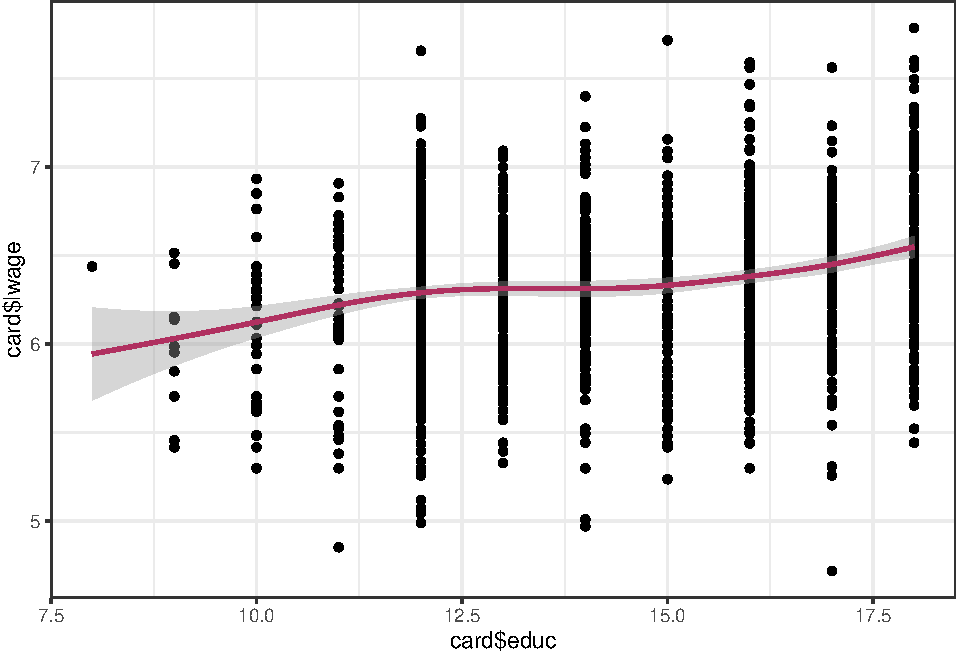
\includegraphics{Assignment-6_files/figure-latex/unnamed-chunk-18-1.pdf}

\begin{Shaded}
\begin{Highlighting}[]
\CommentTok{# There's no clear indicator that the influence of education is non-linear}
\end{Highlighting}
\end{Shaded}

\begin{Shaded}
\begin{Highlighting}[]
\NormalTok{data <-}\StringTok{ }\KeywordTok{read.csv}\NormalTok{(}\StringTok{"EF.csv"}\NormalTok{)}
\CommentTok{# Baseline: Complete randomized experiment}
\NormalTok{Z =}\StringTok{ }\NormalTok{data[,}\DecValTok{1}\NormalTok{]}
\NormalTok{Y =}\StringTok{ }\NormalTok{data[,}\DecValTok{5}\NormalTok{] }\OperatorTok{-}\StringTok{ }\FloatTok{0.75}\OperatorTok{*}\NormalTok{data[,}\DecValTok{4}\NormalTok{] }\OperatorTok{-}\StringTok{ }\FloatTok{0.25}\OperatorTok{*}\NormalTok{data[,}\DecValTok{3}\NormalTok{]}
\CommentTok{# Note that D is not randomized. The difference in means between the treatment and control group is}
\KeywordTok{mean}\NormalTok{(Y[Z }\OperatorTok{==}\StringTok{ }\DecValTok{1}\NormalTok{]) }\OperatorTok{-}\StringTok{ }\KeywordTok{mean}\NormalTok{(Y[Z }\OperatorTok{==}\StringTok{ }\DecValTok{0}\NormalTok{])}
\end{Highlighting}
\end{Shaded}

\begin{verbatim}
## [1] -24.836
\end{verbatim}

\begin{Shaded}
\begin{Highlighting}[]
\CommentTok{# with standard error}
\KeywordTok{sqrt}\NormalTok{(}\KeywordTok{sd}\NormalTok{(Y[Z }\OperatorTok{==}\StringTok{ }\DecValTok{1}\NormalTok{])}\OperatorTok{^}\DecValTok{2} \OperatorTok{/}\StringTok{ }\KeywordTok{length}\NormalTok{(Y[Z }\OperatorTok{==}\StringTok{ }\DecValTok{1}\NormalTok{]) }\OperatorTok{+}\StringTok{ }\KeywordTok{sd}\NormalTok{(Y[Z }\OperatorTok{==}\StringTok{ }\DecValTok{0}\NormalTok{])}\OperatorTok{^}\DecValTok{2} \OperatorTok{/}\StringTok{ }\KeywordTok{length}\NormalTok{(Y[Z }\OperatorTok{==}\StringTok{ }\DecValTok{0}\NormalTok{]))}
\end{Highlighting}
\end{Shaded}

\begin{verbatim}
## [1] 2.655732
\end{verbatim}

\begin{Shaded}
\begin{Highlighting}[]
\CommentTok{# The drug did have a "positive" (in the sense of decreasing cholesterol level) effect.}
\end{Highlighting}
\end{Shaded}

\begin{Shaded}
\begin{Highlighting}[]
\CommentTok{# However, there could be non-compliance. Namely, those assigned to the treatment group do not neccesarily receive enough medicine.}
\CommentTok{# A possible solution is to define the "Compliance Level" as C3 - C4. Those who listens to our advice is more likely to gain a decrease in the cholesterol level. The suggestion was made prior to the treatment assignment. So we can view this either as a covariate or as an instrumental variable.}
\NormalTok{Z =}\StringTok{ }\NormalTok{data[,}\DecValTok{1}\NormalTok{]}
\NormalTok{D =}\StringTok{ }\NormalTok{data[,}\DecValTok{2}\NormalTok{]}
\NormalTok{Y =}\StringTok{ }\NormalTok{data[,}\DecValTok{5}\NormalTok{]}
\NormalTok{X <-}\StringTok{ }\NormalTok{data[,}\DecValTok{3}\NormalTok{] }\OperatorTok{-}\StringTok{ }\NormalTok{data[,}\DecValTok{4}\NormalTok{]}
\CommentTok{# 1. As a covariate, use Lin's regression adjustment}
\NormalTok{model <-}\StringTok{ }\KeywordTok{lm}\NormalTok{(Y}\OperatorTok{~}\StringTok{ }\NormalTok{Z}\OperatorTok{:}\NormalTok{D }\OperatorTok{+}\StringTok{ }\NormalTok{X }\OperatorTok{+}\StringTok{ }\NormalTok{Z}\OperatorTok{:}\NormalTok{D}\OperatorTok{:}\NormalTok{X)}
\NormalTok{model}\OperatorTok{\$}\NormalTok{coef[}\StringTok{"Z:D"}\NormalTok{]}
\end{Highlighting}
\end{Shaded}

\begin{verbatim}
##        Z:D 
## -0.4693973
\end{verbatim}

\begin{Shaded}
\begin{Highlighting}[]
\CommentTok{# The std error estimation is}
\KeywordTok{sqrt}\NormalTok{(}\KeywordTok{hccm}\NormalTok{(model, }\DataTypeTok{type =} \StringTok{"hc0"}\NormalTok{)[}\DecValTok{2}\NormalTok{, }\DecValTok{2}\NormalTok{])}
\end{Highlighting}
\end{Shaded}

\begin{verbatim}
## [1] 0.1426412
\end{verbatim}

\begin{Shaded}
\begin{Highlighting}[]
\KeywordTok{print}\NormalTok{(}\KeywordTok{paste}\NormalTok{(}\StringTok{"One percent of increase in the effective drug intake leads to a decrease of 0.47 in the cholesterol level, assuming unconfoundedness conditioning on the compliance level. The confidence interval is ["}\NormalTok{, model}\OperatorTok{\$}\NormalTok{coef[}\StringTok{"Z:D"}\NormalTok{] }\OperatorTok{-}\StringTok{ }\FloatTok{1.96}\OperatorTok{*}\KeywordTok{sqrt}\NormalTok{(}\KeywordTok{hccm}\NormalTok{(model, }\DataTypeTok{type =} \StringTok{"hc0"}\NormalTok{)[}\DecValTok{2}\NormalTok{, }\DecValTok{2}\NormalTok{]),}\StringTok{","}\NormalTok{,model}\OperatorTok{\$}\NormalTok{coefficients[}\StringTok{"Z:D"}\NormalTok{] }\OperatorTok{+}\StringTok{ }\FloatTok{1.96}\OperatorTok{*}\KeywordTok{sqrt}\NormalTok{(}\KeywordTok{hccm}\NormalTok{(model, }\DataTypeTok{type =} \StringTok{"hc0"}\NormalTok{)[}\DecValTok{2}\NormalTok{, }\DecValTok{2}\NormalTok{]), }\StringTok{"]"}\NormalTok{, }\DataTypeTok{sep =} \StringTok{""}\NormalTok{))}
\end{Highlighting}
\end{Shaded}

\begin{verbatim}
## [1] "One percent of increase in the effective drug intake leads to a decrease of 0.47 in the cholesterol level, assuming unconfoundedness conditioning on the compliance level. The confidence interval is [-0.748974013231253,-0.189820517438327]"
\end{verbatim}

\begin{Shaded}
\begin{Highlighting}[]
\CommentTok{# 2. As an instrumental variable. Then we have to focus on those who receives the real treatment.}
\NormalTok{Z =}\StringTok{ }\NormalTok{data[,}\DecValTok{3}\NormalTok{] }\OperatorTok{-}\StringTok{ }\NormalTok{data[,}\DecValTok{4}\NormalTok{]}
\NormalTok{D =}\StringTok{ }\NormalTok{data[,}\DecValTok{1}\NormalTok{] }\OperatorTok{*}\StringTok{ }\NormalTok{data[,}\DecValTok{2}\NormalTok{]}
\NormalTok{Y =}\StringTok{ }\NormalTok{data[,}\DecValTok{5}\NormalTok{]}
\NormalTok{TSLS_simple <-}\StringTok{ }\ControlFlowTok{function}\NormalTok{(Z, D, Y)\{}
\NormalTok{  D =}\StringTok{ }\KeywordTok{as.matrix}\NormalTok{(D)}
\NormalTok{  Y =}\StringTok{ }\KeywordTok{as.matrix}\NormalTok{(Y)}
\NormalTok{  Z =}\StringTok{ }\KeywordTok{as.matrix}\NormalTok{(Z)}
\NormalTok{  Dhat    =}\StringTok{ }\KeywordTok{lm}\NormalTok{(D }\OperatorTok{~}\StringTok{ }\NormalTok{Z)}\OperatorTok{\$}\NormalTok{fitted.values}
\NormalTok{  tslsreg =}\StringTok{ }\KeywordTok{lm}\NormalTok{(Y }\OperatorTok{~}\StringTok{ }\NormalTok{Dhat)}
\NormalTok{  LATE <-}\StringTok{ }\KeywordTok{coef}\NormalTok{(tslsreg)[}\DecValTok{2}\NormalTok{]}
\NormalTok{  res.correct       =}\StringTok{ }\NormalTok{Y }\OperatorTok{-}\StringTok{ }\KeywordTok{cbind}\NormalTok{(}\DecValTok{1}\NormalTok{, D)}\OperatorTok{\%*\%}\KeywordTok{coef}\NormalTok{(tslsreg)}
\NormalTok{  tslsreg}\OperatorTok{\$}\NormalTok{residuals =}\StringTok{ }\KeywordTok{as.vector}\NormalTok{(res.correct)}
\NormalTok{  stderr <-}\StringTok{ }\KeywordTok{sqrt}\NormalTok{(}\KeywordTok{hccm}\NormalTok{(tslsreg, }\DataTypeTok{type =} \StringTok{"hc0"}\NormalTok{)[}\DecValTok{2}\NormalTok{, }\DecValTok{2}\NormalTok{])}
  \KeywordTok{return}\NormalTok{(}\KeywordTok{list}\NormalTok{(}\StringTok{"LATE"}\NormalTok{ =}\StringTok{ }\NormalTok{LATE, }\StringTok{"se"}\NormalTok{ =}\StringTok{ }\NormalTok{stderr))}
\NormalTok{\}}
\KeywordTok{print}\NormalTok{(}\KeywordTok{paste}\NormalTok{(}\StringTok{"The point estimate of the average causal effect is "}\NormalTok{, }\KeywordTok{TSLS_simple}\NormalTok{(Z, D, Y)}\OperatorTok{\$}\NormalTok{LATE, }\StringTok{" and the CI is ["}\NormalTok{, }\KeywordTok{TSLS_simple}\NormalTok{(Z, D, Y)}\OperatorTok{\$}\NormalTok{LATE }\OperatorTok{-}\StringTok{ }\FloatTok{1.96}\OperatorTok{*}\KeywordTok{TSLS_simple}\NormalTok{(Z, D, Y)}\OperatorTok{\$}\NormalTok{se,}\StringTok{","}\NormalTok{,}\KeywordTok{TSLS_simple}\NormalTok{(Z, D, Y)}\OperatorTok{\$}\NormalTok{LATE }\OperatorTok{+}\StringTok{ }\FloatTok{1.96}\OperatorTok{*}\KeywordTok{TSLS_simple}\NormalTok{(Z, D, Y)}\OperatorTok{\$}\NormalTok{se, }\StringTok{"]"}\NormalTok{, }\DataTypeTok{sep =} \StringTok{""}\NormalTok{))}
\end{Highlighting}
\end{Shaded}

\begin{verbatim}
## [1] "The point estimate of the average causal effect is -1.88023867357047 and the CI is [-3.89355825424121,0.13308090710026]"
\end{verbatim}

\begin{Shaded}
\begin{Highlighting}[]
\CommentTok{# Under 95\% significance level, we do not reject the null hypothesis. For those who receives the real treatment, the concertration/ proportion of the drug have no significant effect on our outcome.}
\end{Highlighting}
\end{Shaded}


\end{document}
